\documentclass[a4paper,fontset=fandol]{ctexart}

\usepackage{amsmath,amssymb,amsthm,physics,fancyhdr,geometry,hyperref,graphicx,enumitem,upgreek,booktabs}

\geometry{vmargin=2cm,hmargin=2.5cm}

\pagestyle{fancy}
\fancyhf{}
\fancyfoot[C]{\thepage}
\renewcommand{\headrulewidth}{0pt}

\usepackage{titlesec}
\titleformat{\section}
{\normalfont\Large\bfseries}{数据分析\thesection:}{0.5em}{}

\newcommand{\points}[1]{\par % 确保换行
	\noindent % 取消缩进
	\hfill (#1分)% 右对齐并添加分数
	\vspace{1em}
}

%\parskip=0.5em

\hypersetup{colorlinks}

\begin{document}
	{
	\Large\bfseries\noindent 数据分析:\hspace{0.5em}指导说明
	}
	
	\begin{itemize}
		\item \textbf{不要触碰信封, 直到考试开始. }
		
		\item 理论考试时长为3小时, 总分为125分.
		
		\item 有\textbf{答题纸}用于详细答题, 以及\textbf{草稿纸}用于粗略计算, 这些纸张已经标记了你的学生代码和题目编号.
		
		\item {\bfseries\itshape 只使用特定题目的答题纸进行答题. 请只在纸张的打印面上书写, 不要使用背面. }如果你在任何纸张上写了不想被评分的内容, 请将其划掉. 
		
		\item 使用尽可能多的数学表达式来帮助评分者更好地理解你的解决方案. 评分者可能不懂你的语言. 如果需要用文字解释某些内容, 请使用简短的短语(如果可能的话, 请使用英语). 
		
		\item 未经允许, 不得离开工作台. 如果你需要任何帮助(计算器故障、需要去洗手间等), 请向监考员示意.
		
		\item 考试的开始和结束将由监考员指示. 剩余时间将在时钟上显示. 
		
		\item 考试结束时, 你必须立即停止书写. 把所有东西放回信封, 并将其留在桌子上. 
		
		\item 一旦收集完所有信封, 你的向导将引导你离开考场. 
		
		\item 信封内附有常数列表和有用的关系式. 
	\end{itemize}
	
	\newpage
	\section{大麦哲伦云的距离}
	
	2019年, 由波兰天文学家领导的国际合作团队以非常高的精确度和准确性测量了大麦哲伦云(LMC)的距离, 它是银河系的一个伴星星系. 通过这种方式, 他们设定了星系际距离尺度的零点, 这使得哈勃常数的测量非常精确. 他们的方法包括测量LMC中20颗食双星的距离, 使用恒星表面亮度$S_V$的概念, 定义为:
	\[S_V=m_V+5\log_{10}\theta,\]
	其中$m_V$是恒星在光学$V$波段的星等, $\theta$是恒星在天空中的角直径, 以毫角秒(mas)为单位. 
	
	量$S_V$可以被理解为角直径为1 mas的恒星的星等. 已知$S_V$和色指数($m_V-m_K$)之间的经验关系, 其中$m_V$和$m_K$分别是$V$波段和红外$K$波段的星等. 下图显示了光谱类型为G和K的巨星的经验关系. 
	
	\begin{figure}[!h]
		\centering
		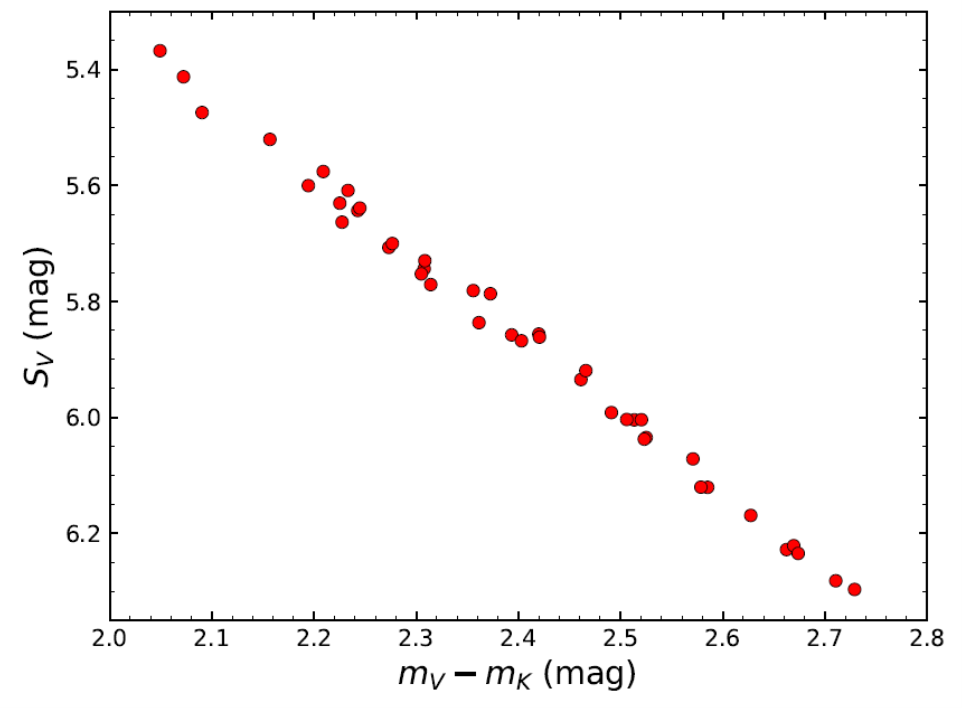
\includegraphics[height=8cm]{fig/1.png}
	\end{figure}
	
	利用这种关系, 可以通过推导食双星系统的物理半径(使用光度测量和光谱学)以及将其与$S_V-(m_V-m_K)$关系预测的角直径进行比较, 来确定食双星系统的距离. 
	
	下表给出了三颗分离食双星的参数. $R_1$和$R_2$是每个子星的半径, $V_{1+2}$和$K_{1+2}$是双星在$V$波段和$K$波段的总亮度(星等), $L_2/L_1$是每个波段中子星的光度比. 
	
	\begin{table}[!h]
		\centering
		\begin{tabular}{|c|c|c|c|c|c|c|}
			\hline
			\textbf{source ID}&$R_1$ [$R_\odot$]&$R_2$ [$R_\odot$]&$V_{1+2}$ [mag]&$K_{1+2}$ [mag]&$L_2/L_1$ ($V$)&$L_2/L_1$ ($K$)\\
			\hline
			OGLE LMC-ECL-03160&17.03&37.42&16.73&14.10&2.80&4.23\\
			\hline
			OGLE LMC-ECL-10567&24.60&36.64&16.15&13.83&1.41&1.99\\
			\hline
			OGLE LMC-ECL-18365&37.30&15.94&16.27&14.01&0.206&0.188\\
			\hline
		\end{tabular}
	\end{table}
	
	将上述方法应用于三个食双星系统, 并计算到大麦哲伦云(LMC)的距离(kpc). 估计结果的总误差. 假设$S_V-(m_V-m_K)$关系的拟合在所有测量中同时引起高达0.8\%的偏差. 
	\points{共50}
	
	\vspace{-1em}
	提示: 在你的计算中, 请保留至少三位有效数字和小数点后两位. 假设星际消光可以忽略不计, 并且大麦哲伦云的角尺寸很小. 
	
	\vspace{1em}
	\section{孤立黑洞}
	
	2022年, 两个独立的研究小组基于对引力微透镜事件OGLE-2011-BLG-0462的观测宣告了孤立黑洞的发现. 在这个问题中, 我们将分析Hubble太空望远镜的数据来复现他们的发现. 
	
	引力微透镜现象发生在一个遥远的恒星(即`源')的光线被一个中间天体(即`透镜')的引力场弯曲并放大时. 引力微透镜事件的特征角尺度, 称为角Einstein半径 $\theta_\mathrm{E}$, 取决于质量 $M$ 和地球到透镜的距离 $D_\ell$:
	\[\theta_\mathrm{E}=\sqrt{\dfrac{4GM}{c^2}\dfrac{D_s-D_\ell}{D_sD_\ell}},\]
	其中 $D_s$ 是到源恒星的距离. 对于在银河系中观察到的典型微透镜事件, 源恒星位于银河系核球处, 靠近银河中心, 所以 $D_s\approx8\text{ kpc}$. 
	
	\begin{enumerate}[label=(\alph*)]
		\item 对于一个质量为1\( M_\odot \)且位于距离地球1 kpc的示例透镜, 计算角Einstein半径, 单位为毫角秒(mas). \hfill(2分)
	\end{enumerate}
	
	假设在时间 \( t \) 时, 透镜和源在天空中的夹角为 \( \theta \equiv u(t)\theta_\mathrm{E} \). 
	在通过光源和透镜位置的一条直线上会产生两个像,它们与透镜的角距离分别为$\theta_+$和$\theta_-$:
	\[\theta_\pm = \dfrac{1}{2}(u \pm \sqrt{u^2 + 4})\theta_\mathrm{E}.\]
	这两个像相对于源的未被透镜作用亮度被放大了. 像的绝对放大率是:
	\[A_\pm = \dfrac{1}{2}\left(\dfrac{u^2 + 2}{u\sqrt{u^2 + 4}} \pm 1\right).\]
	下图展示了该事件的几何结构. 透镜的位置标记为 \( L \), 源的原始位置标记为 \( S \), 而 \( A_+ \) 和 \( A_- \) 标记了源的两个像的位置. 虚线圆的半径为一个Einstein半径. 
	
	\begin{figure}[!h]
		\centering
		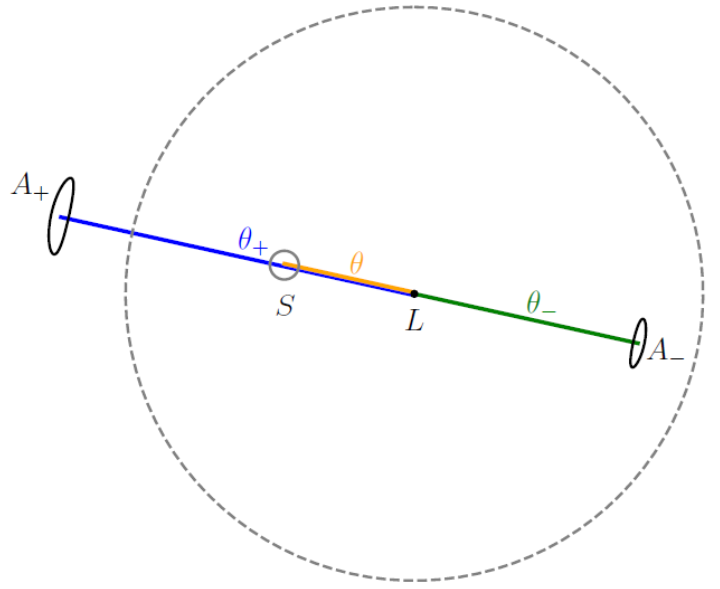
\includegraphics[height=8cm]{fig/2.png}
	\end{figure}
	
	\begin{enumerate}[label=(\alph*),start=2]
		\item 目前的望远镜通常无法分辨这对像, 而只能测量像的中心位置, 即两个像位置的亮度加权平均值. 推导出像中心相对于透镜的角分离 $\theta_c$ 作为 $u$ 和 $\theta_\mathrm{E}$ 的函数的表达式. \hfill(8分)
		
		\item 推导出源的偏转 $\Delta\theta$, 即中心位置与源的原始位置之间的差, 作为 $u$ 和 $\theta_\mathrm{E}$ 的函数的表达式. 当透镜和源几乎完全对齐时($u\approx0$), 源的偏转是多少? \hfill(4分)
	\end{enumerate}
	
	源和透镜在天空中相对于彼此运动. 因此, 像的总放大率和中心的位置都随时间变化, 导致可观测的光度和天体测量微透镜效应. 目前, 我们假设源-透镜相对运动是直线运动. 
	
	下图展示了由华沙大学天文学家领导的OGLE巡天发现的引力微透镜事件OGLE-2011-BLG-0462的光变曲线. 实线显示了最佳拟合的光变曲线模型. 事件的Einstein时间尺度, 即源相对于透镜移动一个角Einstein半径所需的时间, 为 $t_\mathrm{E} = 247\text{ 天}$. 该事件在2011年7月21日(HJD = 2455763)达到峰值. 透镜和源之间的最小分离为 $u_0 \approx 0$. 
	
	\begin{figure}[!h]
		\centering
		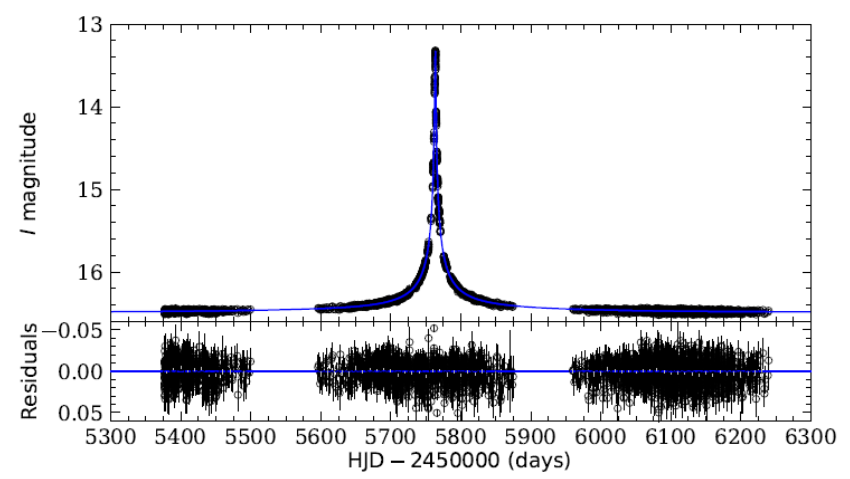
\includegraphics[height=5cm]{fig/3.png}
	\end{figure}
	
	下表展示了基于Hubble太空望远镜图像, 源星相对于背景天体在东和北方向上测量的位置. 
	
	\begin{table}[!h]
		\centering
		\begin{tabular}{rrr}
			\toprule
			HJD&E position (mas)&N position (mas)\\
			\midrule
			2455765.2&$2.58\pm0.13$&$7.29\pm0.16$\\
			2455865.7&$2.32\pm0.12$&$5.44\pm0.24$\\
			2456179.7&$0.46\pm0.14$&$1.62\pm0.08$\\
			2456195.8&$0.88\pm0.36$&$1.56\pm0.77$\\
			2456426.2&$-1.02\pm0.21$&$-0.94\pm0.12$\\
			2456587.7&$-2.04\pm0.07$&$-1.88\pm0.40$\\
			2456956.6&$-4.54\pm0.25$&$-5.16\pm0.29$\\
			2457995.2&$-11.14\pm0.12$&$-15.14\pm0.17$\\
			\bottomrule
		\end{tabular}
	\end{table}
	
	\begin{enumerate}[label=(\alph*),start=4]
		\item 将源星相对于背景天体在东和北方向的测量位置与时间的关系绘制出来. \hfill(10分)
		
		\item 观测到的源星运动是源星的直线自行运动和天体测量微透镜效应的总和. 计算源星在东和北方向的自行(单位为毫角秒/年)及其不确定度. \hfill(8分)
		
		\item 从数据中减去自行效应后, 计算并绘制总天体测量偏转与$u$ 的关系. 忽略自行测定的不确定度. \hfill(20分)
		
		\item 分析数据以确定事件的角Einstein半径 $\theta_\mathrm{E}$ 及其不确定度. (提示: 将 $\Delta\theta$ 的表达式线性化可能很有帮助). \hfill(16分)
		
		\item 对于像OGLE-2011-BLG-0462这样的长时间尺度事件, 透镜-源自行的相对直线运动近似并不严格正确, 必须考虑地球的轨道运动. 这引入测量一个无量纲量, 称为微透镜视差, 定义为 $\pi_\mathrm{E} = (\pi_l - \pi_s) / \theta_\mathrm{E}$, 其中 $\pi_l$ 和 $\pi_s$ 分别是透镜和源的视差. 
		
		对于这个事件, $\pi_\mathrm{E} = 0.095\pm0.009$. 重新写出之前给出的 $\theta_\mathrm{E}$ 表达式, 以计算透镜的质量(单位为太阳质量)及其不确定度. \hfill(7分)
	\end{enumerate}
	\points{共75}
	
\end{document}